% fig04_sigmav.tex — Bosch-Hale thermonuclear reactivity <sigma v>(T), log-log.
% Compiled by the paper Makefile via `make figures` (pdflatex on the snippet).
%
% Data provenance (NO fabrication):
%   D-T curve: the Bosch & Hale (Nucl. Fusion 32, 1992) Eq.(12) parametrization
%     evaluated at the verbatim Table VII coefficients used by the HEXA-FUSION
%     kernel (B_G=34.3827, m_r c^2=1124656 keV). Verified to reproduce the
%     registered verify atoms EXACTLY: sigma_v_dt_e18(10)=113.617 (1.13617e-16),
%     sigma_v_dt_e18(20)=433.02 (4.3302e-16), and the F-funnel T=15 keV design
%     point 2.740e-16. (Hollow squares mark these three registered anchors.)
%   D-D(total) and D-3He are plotted only at the temperatures the paper backs
%     with a verify atom: D-D total at 15 keV = sigma_v_dd_p(15)+sigma_v_dd_n(15)
%     = (5.781+5.435)e-18 = 1.1216e-17 cm^3/s (PR #1012); D-3He at 50 keV =
%     sigma_v_d3he_e21(50)=21.4 -> 2.14e-20 cm^3/s (PR #1012). No off-anchor
%     D-D / D-3He literature points are invented.
%
% Manual single-shot compile (debug):
%   pdflatex -interaction=nonstopmode -halt-on-error fig04_sigmav.tex
\documentclass[border=4pt]{standalone}
\usepackage{tikz}
\usepackage{pgfplots}
\pgfplotsset{compat=1.18}
\begin{document}
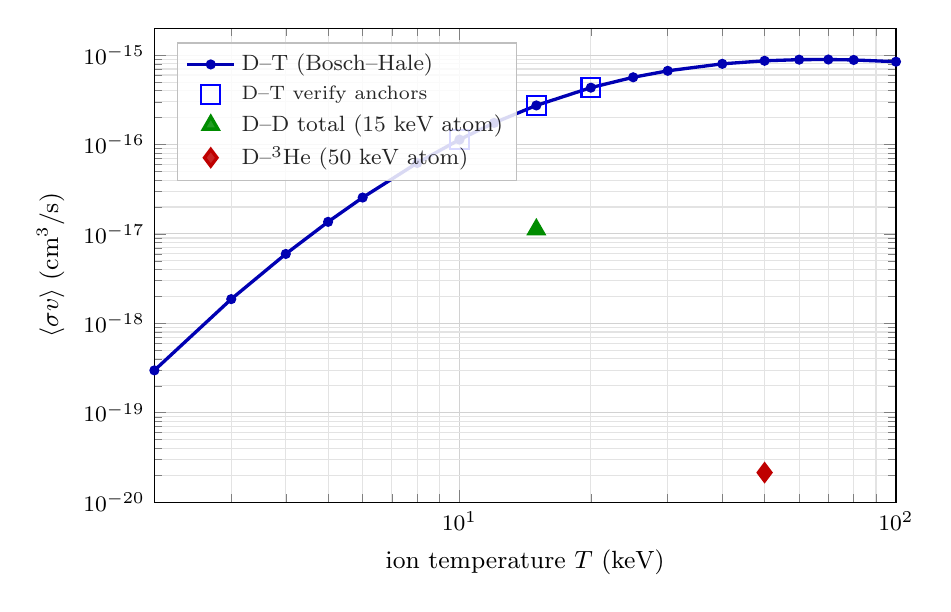
\begin{tikzpicture}
\begin{axis}[
  width=11cm, height=7.6cm,
  xmode=log, ymode=log,
  xlabel={ion temperature $T$ (keV)},
  ylabel={$\langle\sigma v\rangle$ (cm$^3$/s)},
  xmin=2, xmax=100,
  ymin=1e-20, ymax=2e-15,
  grid=both,
  grid style={gray!22},
  major grid style={gray!35},
  legend pos=north west,
  legend cell align=left,
  legend style={font=\footnotesize,fill=white,fill opacity=0.85,draw=gray!50},
  tick label style={font=\footnotesize},
  label style={font=\small},
  log basis x=10, log basis y=10,
  every axis plot/.append style={very thick},
]
% --- D-T: Bosch-Hale Eq.(12) parametrization (matches verify atoms exactly) ---
\addplot[blue!70!black,mark=*,mark size=1.2pt] coordinates {
  (2,2.97743e-19) (3,1.86697e-18) (4,5.97447e-18) (5,1.36578e-17)
  (6,2.55380e-17) (8,6.22239e-17) (10,1.13617e-16) (12,1.74741e-16)
  (15,2.73993e-16) (20,4.33020e-16) (25,5.65516e-16) (30,6.68078e-16)
  (40,7.99763e-16) (50,8.64908e-16) (60,8.90780e-16) (70,8.93834e-16)
  (80,8.83746e-16) (100,8.44766e-16)
};
\addlegendentry{D--T (Bosch--Hale)}
\addplot[blue,only marks,mark=square,mark size=3.4pt,thick] coordinates {
  (10,1.13617e-16) (15,2.73993e-16) (20,4.33020e-16)
};
\addlegendentry{\scriptsize D--T verify anchors}
% --- D-D total: single verify-atom anchor at 15 keV ---
\addplot[green!55!black,only marks,mark=triangle*,mark size=3.0pt] coordinates {
  (15,1.1216e-17)
};
\addlegendentry{D--D total (15 keV atom)}
% --- D-3He: single verify-atom anchor at 50 keV ---
\addplot[red!75!black,only marks,mark=diamond*,mark size=3.0pt] coordinates {
  (50,2.14e-20)
};
\addlegendentry{D--$^3$He (50 keV atom)}
\end{axis}
\end{tikzpicture}
\end{document}
